\section{Novas Funcionalidades e robustez da implementação}


\subsection{Power-ups}

Foram implementados dois tipos de power-up, ambos representados pela classe
abstrata \texttt{PowerUp}, que estende \texttt{Entity} e reutiliza toda a
lógica de movimento já existente na hierarquia, definida por uma velocidade vertical fixa no próprio construtor.

\begin{lstlisting}[caption={\texttt{PowerUp} concentra a coleta em um único método \texttt{final} (PowerUp.java)}]
public abstract class PowerUp extends Entity {
    protected PowerUp(double x, double y, double width, double height, double fallSpeed) {
        super(x, y, width, height);
        setVelocity(0, fallSpeed);
    }

    public final void collectBy(Player player) {
        if (!isActive()) return;

        applyEffect(player);
        deadactivate();
    }

    protected abstract void applyEffect(Player player);
}
\end{lstlisting}

As seguintes regras são comuns a todo power-up e não podem ser alteradas por engano em qualquer sub-classe (por isso o \texttt{final}): 

\begin{itemize}
    \item Um power-up só pode ser coletado uma única vez.
    \item Ele se desativa imediatamente após ser coletado.
\end{itemize}

No entanto, o efeito em si (\texttt{applyEffect}) varia conforme o tipo de power-up. Esses foram os Power-ups implementados:

\begin{itemize}
    \item \textbf{\texttt{ShieldPowerUp}}: Concede ao jogador um escudo
    temporário de 5 segundos, tornando-o invulnerável a qualquer dano. A habilidade
    tem o efeito visual adicional de deixar o player azul, substituindo temporariamente sua cor original.
    \item \textbf{\texttt{TripleShotPowerUp}}: Faz o jogador disparar três
    projéteis em leque (dispersão de 15 graus) a cada tiro, por 8 segundos.
\end{itemize}

Vale notar que a escolha de cada efeito exigiu também a criação de métodos correspondentes na própria
classe \texttt{Player}, responsáveis por ativar, consultar e expirar cada
efeito ao longo do tempo. Exemplo:

\begin{lstlisting}[caption={Métodos adicionados a \texttt{Player} para suportar os efeitos dos power-ups (Player.java)}]
public void activateShield(long durationMs) {
    shieldTimeRemaining = durationMs;
}

public boolean isShielded() {
    return shieldTimeRemaining > 0;
}

public void activateTripleShot(long durationMs) {
    tripleShotTimeRemaining = durationMs;
}

public boolean hasTripleShot() {
    return tripleShotTimeRemaining > 0;
}
\end{lstlisting}

Cada efeito guarda apenas um contador de tempo restante, decrementado a cada
quadro em \texttt{Player.update}, e é consultado no momento certo por outro
método já existente, por exemplo, \texttt{isShielded()} é verificado em
\texttt{takeDamage} (anulando qualquer dano recebido enquanto o escudo estiver
ativo) e \texttt{hasTripleShot()} é verificado em \texttt{tryShoot} (decidindo
se dois projéteis extras em leque devem ser adicionados ao disparo).

\subsection{Chefes de fase}

Foram implementados dois chefes, ambos estendendo a classe abstrata
\texttt{Boss}, que por sua vez estende \texttt{Enemy}. Uma diferença entre os
inimigos comuns e os chefes está no fato em que todo
chefe nasce fora da tela e desliza até uma posição específica da arena antes de assumir
seu comportamento próprio.

\begin{itemize}
    \item \textbf{\texttt{BossType1}} Patrulha
    lateralmente entre dois limites fixos dentro da arena, sem reagir à
    posição do jogador, e dispara periodicamente um leque de três projéteis
    retos para baixo.
    \item \textbf{\texttt{BossType2}}: Descreve um movimento senoidal de
    oscilando verticalmente enquanto deriva lateralmente pela arena, disparando
    um leque de projéteis exatamente uma vez a cada ciclo de mergulho.
\end{itemize}

A classe \texttt{Boss} concentra o comportamento comum de entrada na arena e
delega a cada subclasse apenas o que muda depois disso:

\begin{lstlisting}[caption={\texttt{Boss} decide entre a entrada (comum) e o comportamento próprio de cada chefe (Boss.java)}]
@Override
public void update(long delta) {
    if (updateExploding(delta)) return;

    if (entering) {
        updateEntrance(delta);
    } else {
        super.update(delta);
        updateArenaMovement(delta);
    }
}

// Each boss is responsible for defining its own movement pattern within the screen.
protected abstract void updateArenaMovement(long delta);
\end{lstlisting}

Além disso, \texttt{Boss} sobrescreve dois comportamentos herdados de
\texttt{Enemy}/\texttt{GameObject} para atender aos requisitos específicos de
um chefe de fase: \texttt{isOutOfBounds} sempre retorna \texttt{false} (um
chefe nunca é desativado por sair da tela), e \texttt{diesOnPlayerContact}
também retorna \texttt{false} (diferentemente dos inimigos comuns, um chefe só
pode ser derrotado atirando nele, nunca por colisão direta). 

Ademais, A vida do chefe é
exibida através de uma barra de vida (\texttt{HealthBar}) enquanto ele estiver
ativo em cena, aparecendo e sumindo junto com ele.

\subsection{Sistema de fases (\texttt{GameConfigParser} e \texttt{PhaseConfigParser})}

O jogo é configurado por dois níveis de arquivo texto, lidos em tempo de
execução. Um arquivo principal, definindo a vida do jogador e a lista de
arquivos de fase, e um arquivo por fase, definindo os inimigos, power-ups e o
chefe daquela fase (como consta no próprio enunciado). 

\begin{figure}[H] % ou [htbp]
    \centering
    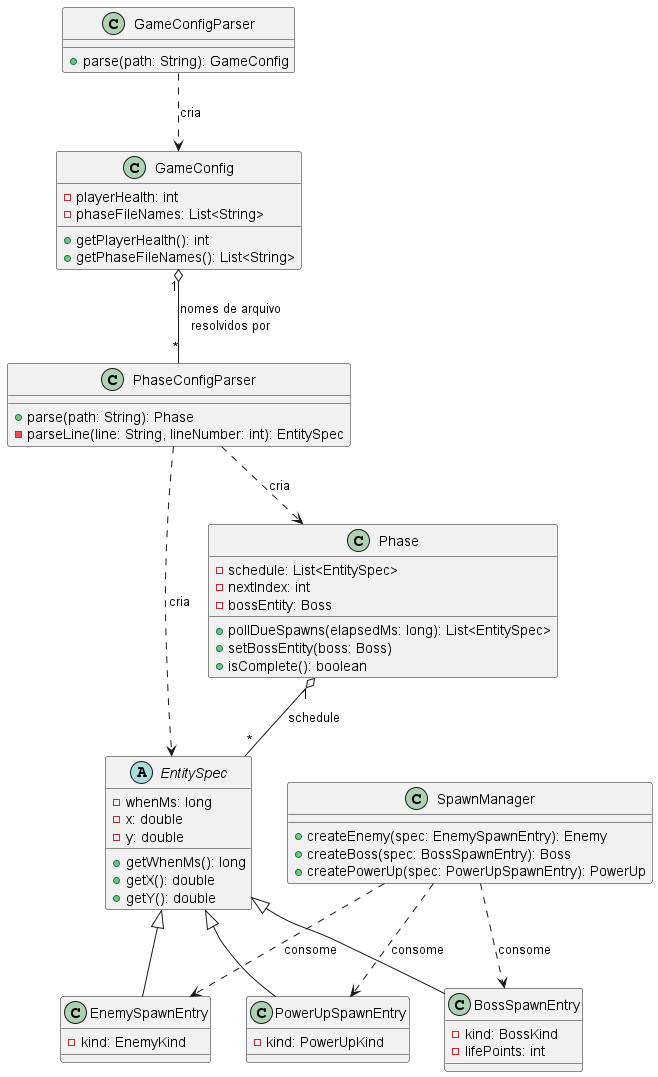
\includegraphics[width=0.4\textwidth]{images/sistema_de_fases.png}
    \caption{Diagrama do sistema de fases}
    \label{fig:sistema_fasess}
\end{figure}

A leitura desses arquivos é feita pelas classes
\texttt{GameConfigParser} e \texttt{PhaseConfigParser}, que traduzem cada
linha em um objeto do tipo \texttt{EntitySpec} (com as subclasses
\texttt{EnemySpawnEntry}, \texttt{BossSpawnEntry} e \texttt{PowerUpSpawnEntry}),
unificando os três tipos de entrada em uma única representação.

A tradução desses dados declarativos em entidades de fato jogáveis é
responsabilidade da classe \texttt{SpawnManager}, com métodos \texttt{createBoss},
\texttt{CreatePowerUp} e \texttt{CreateEnemy}.

Dessa forma, o restante do jogo (a classe \texttt{Game}) precisa apenas consultar o
\texttt{SpawnManager} com o \texttt{EntitySpec} lido do arquivo de
configuração, e a instância concreta correta é devolvida.

\subsection{Robustez do código (exceções e logging)}

A leitura dos arquivos de configuração citado na sessão anterior é o ponto do projeto com maior
exposição a erros em tempo de execução. Por isso, o módulo de
configuração (\texttt{game.config} e seus subpacotes) foi tratado com atenção
especial, combinando exceções descritivas com o uso de
\texttt{java.util.logging} para registrar o que aconteceu.

\subsubsection{Exceções}

Sempre que uma linha de um arquivo de configuração está malformada, o parser
correspondente lança uma exceção com uma mensagem específica, indicando
exatamente qual campo é o problema. Exemplo:

\begin{lstlisting}[caption={Exceções descritivas (GameConfigParser.java)}]
private int parseIntline(String line, String description){
    if (line == null)
        throw new IllegalStateException("Arquivo de configuração incompleto: faltando " + description + ".");

    try {
        return Integer.parseInt(line.trim());
    } catch (NumberFormatException e) {
        throw new IllegalStateException("Valor inválido para " + description + ": \"" + line + "\"", e);
    }
}
\end{lstlisting}

Essas exceções, no entanto, são tratadas de duas formas diferentes dependendo
da sua gravidade, o que evita que um erro pontual derrube o jogo inteiro
desnecessariamente. Uma entrada isolada malformada dentro de um arquivo de
fase (um \texttt{INIMIGO} ou \texttt{POWERUP} com tipo
desconhecido/fora do padrão, por exemplo) é simplesmente ignorada, registrando um aviso e
permitindo que o restante da fase continue normalmente, como mostra:

\begin{lstlisting}[caption={Uma entrada inválida não derruba a fase inteira (Game.java)}]
private void spawnDueEntities() {
    List<EntitySpec> due = currentPhase.pollDueSpawns(phaseElapsedMs);

    for (EntitySpec spec : due) {
        try {
            spawnEntity(spec);
        } catch (IllegalArgumentException e) {
            // a single malformed/unknown entry in the phase file shouldn't take
            // the whole game down; skip it and keep playing.
            LOGGER.log(Level.WARNING, "Skipping invalid spawn entry: " + spec, e);
        }
    }
}
\end{lstlisting}

Já uma falha estrutural mais grave, como o próprio arquivo de configuração
principal não sendo encontrado, é trata como fatal em um único ponto
central, no laço principal do jogo, evitando que a aplicação trave com uma
janela aberta e sem nenhuma explicação visível ao usuário.

\begin{lstlisting}[caption={Falhas fatais são registradas e encerram o jogo (Game.java)}]
try {
    ...
} catch (Exception e) {
    // last resort: without this, a startup/runtime failure would crash the thread
    // after initGraphics() already opened the window, leaving a frozen,
    // never-drawn screen with no visible clue why
    LOGGER.log(Level.SEVERE, "Fatal error, aborting game.", e);
}
\end{lstlisting}

\subsubsection{Logging}

O uso do \texttt{Logger} (de \texttt{java.util.logging}) contribui para uma melhor
organização das informações geradas durante a execução do programa. Em vez de
exibir todas as mensagens da mesma forma, o sistema permite classificá-las de
acordo com sua importância, facilitando a identificação de eventos relevantes e
de possíveis problemas.

Além de auxiliar durante o desenvolvimento e os testes, o uso de \textit{logging}
é considerado uma boa prática em projetos de software, pois torna a manutenção
mais simples e o acompanhamento do comportamento da aplicação mais eficiente.
Dessa forma, informações importantes podem ser registradas sem comprometer a
clareza da saída principal do jogo, mantendo a experiência do usuário mais
organizada e facilitando futuras correções ou melhorias.
